\lecture{10}{26 marzo 2024}
\section{Onde sonore}


Le onde sonore viaggiano in generale in tre dimensioni, oggi ci limiteremo al caso unidimensionale facendole viaggiare in un tubo. Le onde sulla corda sono trasversali rispetto alla direzione di propagazione dell'onda, esse hanno bisogno di qualcosa di solido per propagarsi perché sono necessari dei vincoli sulle posizioni dei punti. Nei liquidi e nei gas le onde trasversali non sono quindi possibili, mentre avvengono onde longitudinali (oscillazione nella stessa direzione del moto).
Se ho una direzione di propagazione ben precisa le onde sono trattabili a tutti gli effetti come onde scalari.
\begin{figure}[H]
	\centering
	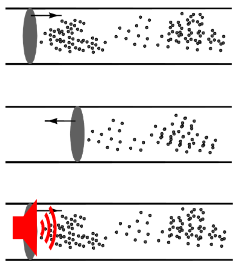
\includegraphics[width=0.2\textwidth]{screenshots/2024-03-26-11-17-49.png}
	\caption{Tubo riempito di gas e membrana che possa comprimere o decomprimere il gas. La membrana può essere immaginata come un semplice speaker.}
\end{figure}
L'attivazione del pistoncino provoca variazioni di pressione e quindi di densità del gas. Pongo un sistema di riferimento con \(x=0\) sulla membrana e studio il comportamento del tubo.
\begin{figure}[H]
	\centering
	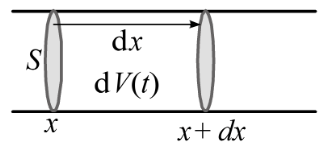
\includegraphics[width=0.4\textwidth]{screenshots/2024-03-26-11-21-58.png}
\end{figure}
Mi limito a una zona del tubo \([x, x+ \mathrm{d} x]\) limitata da due diaframmi senza massa e mobili. La massa \(\mathrm{d} m\) del gas occupa nel tempo volumi diversi, ma è una costante. Inizialmente \(\mathrm{d} m = \rho _0 D \mathrm{d} x\). Successivamente il gas viene compresso e i due diaframmi si muovono.
\begin{figure}[H]
	\centering
	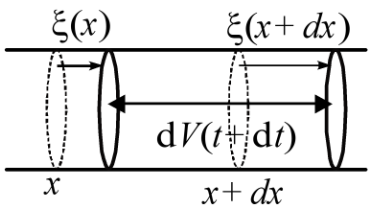
\includegraphics[width=0.4\textwidth]{screenshots/2024-03-26-11-25-08.png}
\end{figure}
Quindi ho che
\begin{gather}
	\mathrm{d} V(t) = S [\mathrm{d} x + \xi (x + \mathrm{d} x) - \xi (x)]=S \mathrm{d} x \left[ 1 + \left( \frac{\partial \xi }{\partial x}  \right)_x  \right]\\
	\mathrm{d} m = cost. \implies \rho _0 S \mathrm{d} x = \rho S \mathrm{d} x \left[ 1+ \left( \frac{\partial \xi }{\partial x}  \right)_x \right]\\
	\rightsquigarrow \frac{\rho}{\rho _0} = \frac{1}{1+ \left( \frac{\partial \xi }{\partial x}  \right)_x}
\end{gather}
Ora posso espandere per piccole perturbazioni:
\begin{gather}
	\frac{\rho }{\rho _0} = \left[1+ \left( \frac{\partial \xi }{\partial x}  \right)_x  \right] ^{-1} \thickapprox 1 - \left( \frac{\partial \xi }{\partial x}  \right)_x\\
	\rightsquigarrow \rho (x,t) - \rho _0 = - \rho _0 \left( \frac{\partial \xi }{\partial x}  \right)_x 
\end{gather}
Studiamo la dinamica del volumetto sull'asse x. \(a_x = \frac{\partial ^{2} \xi }{\partial t ^{2} } \). Sia \(p(x)\) la pressione.
\begin{equation}
	F_x = p(x)S - p(x+ \mathrm{d} x)S
\end{equation}
Proseguendo con i calcoli si ottiene che
\begin{figure}[H]
	\centering
	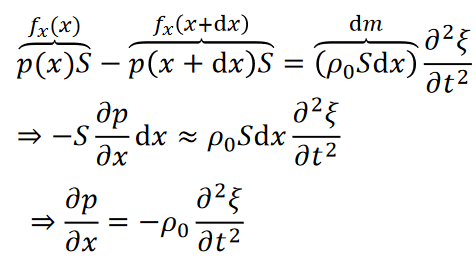
\includegraphics[width=0.4\textwidth]{screenshots/2024-03-26-11-36-18.png}
\end{figure}
Ho collegato una variazione del gas (pressione) a una variazione del mio volumetto. Quindi le onde sonore cambiano la pressione \(p(x)\) e la densità \(\rho (x)\). Adesso studio la variazione di \(p(\rho )\) in prossimità della condizione di equilibrio \((P_0=p(\rho _0), \rho _0)\):
\begin{equation}
	p(\rho )\thickapprox P_0 + \left. \frac{\partial p}{\partial \rho } \right| _{\rho = \rho _0}(\rho - \rho _0) = P_0 + \frac{\beta }{\rho _0}(\rho - \rho _0) = P_0 - \beta \left( \frac{\partial \xi }{\partial x}  \right) _x
\end{equation}
Devo capire quanto vale \(\beta / \rho _0\). Possiamo assumere che il gas faccia una trasformazione adiabatica, perché le trasformazioni che comportano un passaggio di calore sono molto lente e le onde sonore sono invece molto veloci. Grazie a questa considerazione possiamo scrivere \(p(\rho ) = \alpha \rho ^\gamma \).
\begin{gather}
	\beta = \rho _0 \left. \frac{\partial p}{\partial \rho } \right| _ {\rho = \rho _0} = \rho _0 \gamma \alpha \rho _0 ^{\gamma -1} = \gamma \alpha \rho _0 ^\gamma = \gamma P_0\\
	p(x) = P_0 - \beta \left( \frac{\partial \xi }{\partial x}  \right) _x \rightsquigarrow \frac{\partial p}{\partial x} = - \beta \left( \frac{\partial ^{2} \xi }{\partial x^{2} }  \right) _x
\end{gather}
Da cui si ottiene un'equazione di D'Alembert:
\begin{figure}[H]
	\centering
	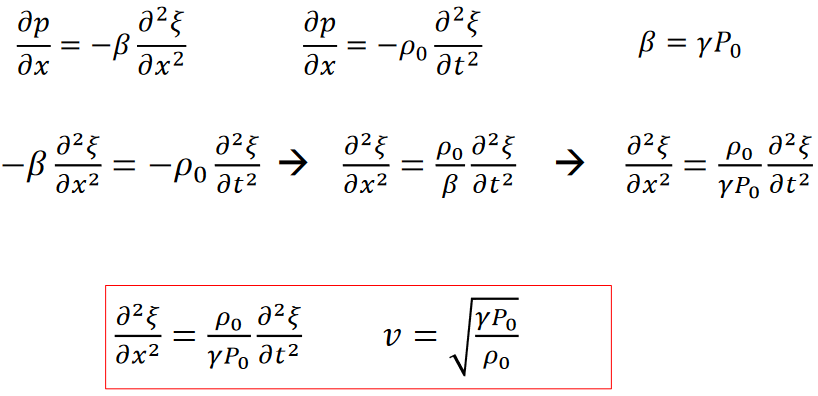
\includegraphics[width=0.6\textwidth]{screenshots/2024-03-26-11-51-20.png}
\end{figure}
Le soluzioni sono le stesse di quelle viste sulla corda! In particolare, avremo onde regressive e progressive.
\begin{eg}
	Verifichiamo la previsione teorica della velocità del suono considerando l'aria secca a livello del mare: \(P_0 = 1.015 \times 10^5 \unit{Pa},\ \rho _0 = 1.29 \unit{kg/ m^3 }\). \(\gamma \) è praticamente 1.4 perché l'aria è principalmente un gas biatomico (azoto e ossigeno).
	\begin{equation}
		v_{teo} = \sqrt{\frac{\gamma P_0}{\rho _0}} = 331 \unit{m/s} \hspace{1cm} v_{mis} = 330 \unit{m / s} 
	\end{equation}
	C'è un accordo entro il 3 per mille! Significa che le approssimazioni che abbiamo fatto sono valide e funzionano molto bene. In acqua la velocità è di circa \(1400 \unit{m / s}\), nel granito è circa \(6000 \unit{m /s}\).
\end{eg}

\paragraph{Cosa sono le onde sonore?}
Sono onde di spostamento della posizione delle molecole \(\xi (x,t)\):
\begin{equation}
	\frac{\partial^{2}  \xi }{\partial x^{2} } = \frac{\rho _0}{\gamma P_0} \frac{\partial ^{2} \xi }{\partial t ^{2} }  
\end{equation}
Ma sono anche onde di densità \(\rho (x,t)\):
\begin{equation}
	\rho (x,t) = \rho _0 - \rho _0 \frac{\partial \xi }{\partial x} \rightsquigarrow \frac{\partial ^{2} \rho }{\partial x^{2} } = \frac{\rho _0}{\gamma P_0} \frac{\partial ^{2} \rho }{\partial t ^{2} }  
\end{equation}
E anche onde di pressione \(p(x,t)\):
\begin{equation}
	p(x,t) = P_0 - \gamma P_0 \frac{\partial \xi }{\partial x} \rightsquigarrow \frac{\partial ^{2} p}{\partial x^{2} } = \frac{\rho _0}{\gamma P_0} \frac{\partial ^{2} p}{\partial t ^{2} }  
\end{equation}

\subsection{Analisi energetica delle onde sonore}

Il diaframma applica una forza sul gas data da \(F_x = S p(x,t)\), quindi il suo lavoro risulta \(\delta L = F_x \mathrm{d} x = S p(x,t) \dot{\xi }(x,t) \mathrm{d} t\), quindi
\begin{figure}[H]
	\centering
	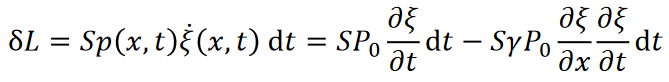
\includegraphics[width=0.6\textwidth]{screenshots/2024-03-26-12-16-55.png}
\end{figure}
Dividendo per il tempo otteniamo la potenza:
\begin{figure}[H]
	\centering
	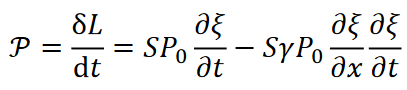
\includegraphics[width=0.5\textwidth]{screenshots/2024-03-26-12-17-38.png}
\end{figure}
Il primo termine ha media nulla perché la media dello spostamento spaziale nel tempo è nulla, quindi il primo termine non è un'energia associata all'onda perché non viaggia. L'unico termine che ci interessa è il secondo, che rappresenta l'energia effettivamente immessa nel tubo e che ha la possibilità di propagarsi:
\begin{figure}[H]
	\centering
	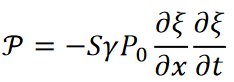
\includegraphics[width=0.3\textwidth]{screenshots/2024-03-26-12-20-51.png}
\end{figure} 
È proporzionale alla sezione del tubo, questo ci torna comodo perché in generale quando parliamo di intensità vogliamo una quantità definita punto per punto e non su una superficie. Quindi definisco l'intensità delle onde sonore.
\begin{definition}
	[Intensità di onda sonora]
	Si definisce intensità di onda sonora:
	\begin{equation}
		I = \left\langle \frac{\mathcal{P} }{S} \right\rangle = \left\langle -\gamma P_0 \frac{\partial \xi }{\partial x} \frac{\partial \xi }{\partial t}  \right\rangle 
	\end{equation}
	È una quantità puntuale e si misura in \unit{W / m^2}.
\end{definition}
Per le onde progressive la derivata spaziale è proporzionale alla derivata temporale, quindi posso scrivere
\begin{equation}
	I \left\langle \frac{\gamma P_0}{v} \left( \frac{\partial \xi }{\partial t}  \right) ^{2}   \right\rangle = \left\langle v \gamma P_0 \left( \frac{\partial \xi }{\partial x}  \right)^{2}   \right\rangle 
\end{equation}
\begin{definition}
	[Impedenza acustica specifica]
	Si definisce l'impedenza acustica specifica:
	\begin{equation}
		Z = \frac{\gamma P_0}{v} = \sqrt{\gamma P_0 \rho _0} 
	\end{equation}
\end{definition}
Utilizzando l'impedenza appena definita si scrive che
\begin{equation}
	I = \left\langle Z \left( \frac{\partial \xi }{\partial t}  \right) ^{2}  \right\rangle,
\end{equation}
% TODO: aggiungi ref a equazione corda
che ha una forma identica a quella che compariva sulla corda, ma con diverse unità di misura!
\paragraph{Impedenza come causa-effetto}
Avevamo già detto che l'impedenza compariva come costante di proporzionalità fra una causa e il suo effetto. Cerchiamo una relazione di questo tipo in questo caso. Ricordiamo che
\begin{gather}
	p(x,t) = P_0 - \gamma P_0 \frac{\partial \xi }{\partial x}\\
	\delta p = - \gamma P_0 \frac{\partial \xi }{\partial x} = \frac{\gamma  P_0}{v} \frac{\partial \xi }{\partial t} = Z \frac{\partial \xi }{\partial t} 
\end{gather}
dove la variazione di pressione è la causa dello spostamento del gas.

\paragraph{Come udiamo il suono}
Il nostro timpano si comporta esattamente come un oscillatore armonico forzato all'arrivo di un'onda sonora. Possiamo immaginarlo come un oscillatore con un fattore di qualità molto piccolo, perché il timpano è sensibili a frequenze fra \(20 \unit{Hz}\) e \(20000 \unit{Hz}\). La massima sensibilità è attorno ai \(2-3 \unit{kHz}\), le frequenze della voce stanno fra i \(20 \unit{Hz}\) e i \(4 \unit{kHz}\). L'intensità minima percepibile è \(I_0 = 10^{-12} \unit{W / m^2}\) e la soglia del dolore è convenzionalmente definita come \(I_{dol} = 1 \unit{W / m^2}\). L'intensità massima, che provoca un immediato danno meccanico all'orecchio, è \(I_{max} = 10 \unit{W / m^2}\). Questi valori sono convenzionalmente assegnati perché poi in realtà variano in base alla frequenza del suono e da persona a persona.
\begin{figure}[H]
	\centering
	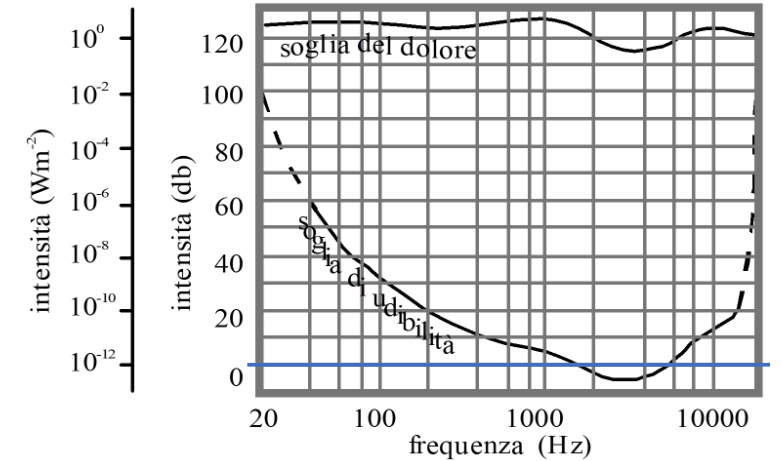
\includegraphics[width=0.6\textwidth]{screenshots/2024-03-26-12-39-25.png}
\end{figure}
L'intervallo di intensità sonora in cui l'orecchio umano è sensibile è enorme: tredici ordini di grandezza! Per questo motivo è più comodo studiarla in scala logaritmica, definendo il livello sonoro in deciBel:
\begin{equation}
	\beta _s = 10 \log_{10} \left( \frac{I}{I_0} \right) \unit{dB}
\end{equation}
Di conseguenza, il limite di udibilità è \(\beta _s = 0 \unit{dB}\), la soglia del dolore \(\beta _s = 120 \unit{dB}\) e il danno permanente immediato a \(\beta _s = 130 \unit{dB}\).

\paragraph{Giustificazione delle approssimazioni}
Calcoliamo l'intensità e l'ampiezza delle oscillazioni delle molecole d'aria con un suono armonico di frequenza \(f= 1 \unit{kHz}\), livello sonoro \(\beta _s = 50 \unit{dB}\) e in aria standard:
\begin{figure}[H]
	\centering
	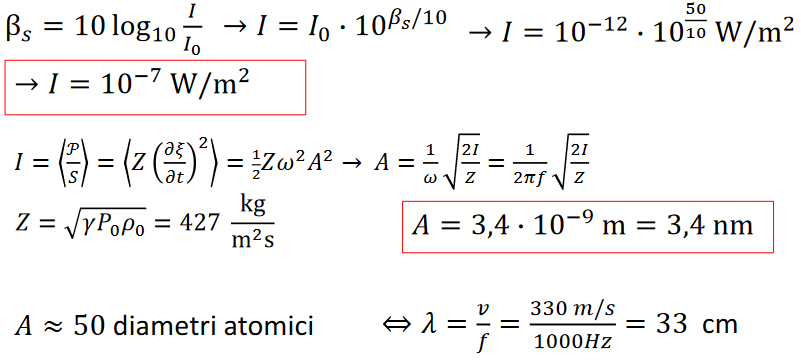
\includegraphics[width=0.7\textwidth]{screenshots/2024-03-26-12-45-53.png}
\end{figure}
Si nota che l'ampiezza delle oscillazioni è molto inferiore rispetto alla lunghezza d'onda del suono. Si nota lo stesso fatto anche per le variazioni di densità e di pressione:
\begin{figure}[H]
	\centering
	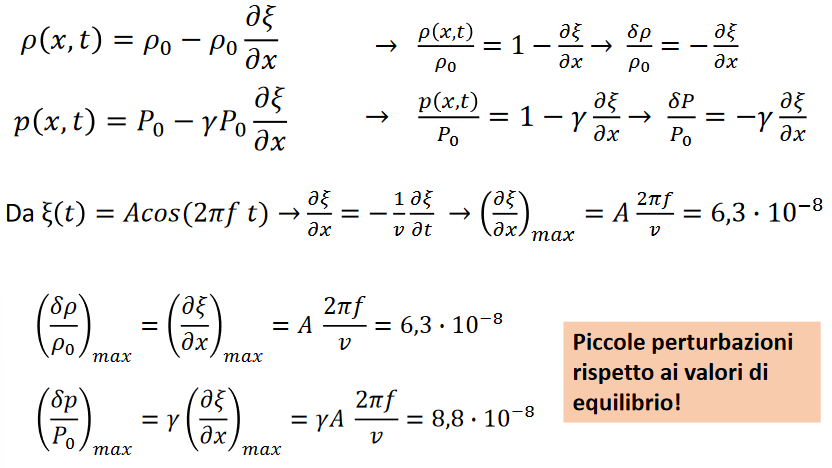
\includegraphics[width=0.7\textwidth]{screenshots/2024-03-26-12-49-46.png}
\end{figure}
Essendo tutte variazioni molto piccole, le equazioni di D'Alembert sono quelle \emph{corrette} per le onde sonore, pur avendo applicato alcune approssimazioni al nostro modello. Questo significa che tutte le onde viaggiano alla stessa velocità (per fortuna, altrimenti sentiremmo la musica diversamente a seconda della distanza dalla sorgente!).